\documentclass[12pt]{article}
\usepackage[a4paper, hmargin={2.5cm, 2.5cm}, vmargin={2.5cm, 2.5cm}]{geometry}
\linespread{1.5}
\usepackage{eso-pic} % \AddToShipoutPicture
\usepackage{graphicx} % \includegraphics
\usepackage[utf8]{inputenc}
\usepackage[danish]{babel}
\usepackage[T1]{fontenc}
\usepackage{hyperref}
\usepackage{amsmath, amscd}
\usepackage{amsmath,amscd}
\usepackage{amssymb}
\usepackage{amsthm}
\usepackage{enumerate}
\usepackage{graphicx}
\usepackage{framed}
\usepackage{color}
\usepackage{listings}
\usepackage{float}
\usepackage{dirtree}
%\usepackage[none]{hyphenat}
\usepackage[super]{cite}
\lstset{
	frame=single,
	breaklines=true,
	postbreak=\raisebox{0ex}[0ex][0ex]{\ensuremath{\color{red}\hookrightarrow\space}}
}
\newcounter{nodeCdepth}
\newenvironment{nodeC}
{\ifnum\value{nodeCdepth}=0
    \gdef\listfordirtree{}%
    \let\item\nodeCitem
    \fi
    \stepcounter{nodeCdepth}}
{\addtocounter{nodeCdepth}{-1}%
    \ifnum\value{nodeCdepth}=0
    \expandafter\dirtree\expandafter{\listfordirtree}%
    \fi}
\newcommand{\nodeCitem}[1]{%
    \xdef\listfordirtree{%
        \unexpanded\expandafter{\listfordirtree}%
        .\thenodeCdepth\space\unexpanded{#1}. }%
}
%% Change `ku-farve` to `nat-farve` to use SCIENCE's old colors or
%% `natbio-farve` to use SCIENCE's new colors and logo.
\def \ColourPDF {../include/ku-farve}

%% Change `ku-en` to `nat-en` to use the `Faculty of Science` header
\def \TitlePDF {../include/ku-en}  % University of Copenhagen

\title{
  \vspace{3cm}
  \Huge{Eksamensrapport} \\
  \Large{Software Udvikling 2016 - Project-Stock}
	}

\author{
	\Large{Stefan Friis Tofte} - \textbf{jwr342} - \texttt{stefan.f.tofte@gmail.com}
	\and
	\Large{Mads Kronborg} - \textbf{xlq446} - \texttt{kronborg96@gmail.com}
	\and
	\Large{Lasse Halberg Haarbye} - \textbf{lpt113} - \texttt{ninjalf2@gmail.com}
	\and
	\Large{Christian E.N. Hansen} - \textbf{vmk541} - \texttt{cralle@outlook.com}
}


\begin{document}


\AddToShipoutPicture*{\put(0,0){\includegraphics*[viewport=0 0 700 600]{\ColourPDF}}}
\AddToShipoutPicture*{\put(0,602){\includegraphics*[viewport=0 600 700 1600]{\ColourPDF}}}

\AddToShipoutPicture*{\put(0,0){\includegraphics*{\TitlePDF}}}

\clearpage\maketitle
\thispagestyle{empty}

\newpage
\tableofcontents
\newpage

\section{Indledning}
\label{sec:indledning}
Hvert år skal datalogistuderende på DIKU finde et projekt til at afslutte deres bachelor eller kandidat. Det kan være en besværlig proces at finde en vejleder eller et emne som passer til ens ønsker. De studerende har enten skulle gå fra dør til dør og spørge en vejleder, om de har et projekt til en eller være tilstede til en enkel forelæsning hvor nogle vejledere præsenterer deres projekter. \\ \\
Vi som studerende har en vis interesse i at få et bedre system på plads, hvori studerende kan finde et katalog med vejledere og projekter, da vi selv kommer til at stå i en situation hvor vi skal finde et kandidat eller bachelor projekt. En måde at se hvilke projekter vejlederne har liggende, men også en mulighed for at se hvilke projekter de har haft tidligere. \\ \\
Vores løsning til dette problem er en dynamisk hjemmeside, hvori vejledere selv kan ligge projekter op, informere om deadlines og meget andet. Hjemmesiden er skrevet i det objektorienterede programmeringssprog \textit{Python} samt open-source frameworket \textit{Django}. \\ \\
Vi vil igennem rapporten gå igennem de krav vi har opstillet, vores designproces, afprøvning, udviklingsmiljø, og til sidst vil vi diskutere, hvad der mangler at blive lavet på vores projekt og hvordan vi har arbejdet sammen.\\

\section{Problembeskrivelse}
\label{sec:problem}
Vores projekt er udviklet som en løsning på den til dels besværlige proces, som det kan være at tilmelde sig bachelorprojekter. Jyrki, som er medansvarlig for bachelorprojekterne, ønskede en mindre manuel løsning end den forhenværende. Det største problem i den tidligere løsning opstod når elever skulle gå fra professor til professor og få afslag. Yderligere har problemer som den nye reform gjort det endnu vigtigere at få en hurtigere og smartere metode. \\
Vi har derfor lavet en side, som ved automatisk \textit{scraping}\cite{scraping} af informationer fra DIKU's hjemmeside, kan præsentere en opdateret visning af de forskellige ledige projekter og vejledere, samt deres arbejdsbyrde. Opsumeret har vi altså fået implementeret alle "Quality requirements". \\
% mellemrum efter " bliver slettet, derfor {}
Vi kunne til gengæld ikke opfylde alle de funktionelle krav, da et punkt som f.eks. "There should be a mechanism to check the quality of industrial projects"{} er for subjektivt og vi hverken har erfaring eller viden omkring dette. \\
Ligeledes har vi også valgt ikke at implementere en løsning, hvor studerende kan lave et "ønske-opslag"{} om uaktuelle emner, i håb om at nogle vejledere vil lave et projekt om det.

\section{Krav}
\label{sec:krav}
I forløbets start opstillede vi nogle \textit{use cases}, for at imødekomme de krav vores \textit{product owner} havde til det produkt, vi skulle udvikle. \\
Vi foretog en løs priotering af produktets use cases og vurderede, hvad der var kernefunktionaliteter, og hvad der var \textit{"nice-to-have"}-funktionaliteter.

\subsection*{Use cases}

\subsubsection{Kernefunktionaliteter}
\label{sec:corefuncs}
\begin{enumerate}
	\item Det skal være muligt at se et katalog over projekter.
	\item Systemet skal kunne præsentere opdaterede oplysninger om potentielle vejledere, herunder:
	\begin{itemize}
		\item Tidligere projekter
		\item Forskningspublikationer
		\item Kontaktoplysninger
	\end{itemize}
	\item Personer, der optræder på siden, skal kunne verificeres, hvis de eksempelvis ønsker at tilføje projekter eller foretage rettelser.
\end{enumerate}

\subsubsection{"Nice-to-have"{}-funktionaliteter}
\label{sec:nicefuncs}
\begin{enumerate}
  \item Systemet skal kunne vise projekter knyttet til specifikke keywords.

  \item Systemet skal vise en status på en vejleders arbejdsbyrde.
  \item En vejleder eller en person knyttet til en \textit{business-club}, skal kunne tilføje et projekt til projektkataloget.

	\item Systemet skal kunne filtrere vejledere i forhold til keywords i forskningspublikationer (titler).
\end{enumerate}


\section{Design}
\label{sec:design}
% Lasse
\subsection{Generelt om Django frameworket}
\label{sec:genereltdjango}
Django frameworket er opbygget efter designmønstret \textit{Model-View-Controller (MVC)}. Udviklerne har dog valgt navnekonventionen \textit{Model-Template-View (MTV)} \cite{djangoFAQ}. I Django kan man tilgå og validere data fra f.eks. en database vha. \textit{models}\cite{models}. Her kan Django frameworket hjælpe således, at et felt i Django-model svarer til et felt i en databasetabel. \\
Et \textit{view}\cite{djangoView} er en Python-funktion, der tager en web-forespørgsel og returnerer en web-respons i form af HTML som kan vises til brugeren. \\
\textit{Templates} (skabeloner) benyttes til dynamisk at genere HTML-sider, for at spare kode og for nemt at kunne benytte variabelnavne, direkte i det HTML brugeren får vist i sin browser. Django har sit eget indbyggede template sprog\cite{djangoTemplate}, som vi har benyttet i vores projekt.\\
\\
Djangos filstruktur er beskrevet i sektion \hyperref[sec:struktur]{\ref*{sec:struktur}: \nameref*{sec:struktur}}.

\subsection{Struktur}
\label{sec:struktur}
Et Django-projekt har en struktur der ser således ud:\\
\begin{nodeC}
    \item{project\_stock}
    \begin{nodeC}
        \item{manage.py}
        \item{project\_stock}
        \begin{nodeC}
            \item{\_\_init\_\_py}
            \item{apps.py}
            \item{models.py}
            \item{settings.py}
            \item{tests.py}
            \item{urls.py}
            \item{views.py}
            \item{wsgi}
        \end{nodeC}
    \end{nodeC}
\end{nodeC}~\\
Nogle af disse filer er vigtigere end andre for at have en tilgængelig webapplikation, bl.a. settings.py, der definerer projektets indstillinger, urls.py, der definerer hvilke URL's som brugere kan tilgå og views, der definerer hvad brugeren kommer til at se.\\
\\
% Forklaring følger
Filen \texttt{manage.py} er essentiel eftersom, at det er den fil som styrer selve hjemmesiden. Det er med den fil man opretter et Django-projekt, starter en lokal webserver, opdaterer ens database og meget andet.\\
Vi har en fil der hedder \texttt{fillmockdata.py}, som står for at bruge scraperen til at høste data, hvorefter den indsætter det i databasen. Det er altså et interface mellem scraperen og det Django-specifikke databasekode.\\
\\
<<<<<<< HEAD
Vores specifikke struktur kan findes i bilag under ...

\subsection{Generelt om Django frameworket}
Django frameworket er opbygget efter designmønstret \textit{Model-View-Controller (MVC)}. Udviklerne har dog valgt navnekonventionen \textit{Model-Template-View (MTV)} \cite{djangoFAQ}. I Django er \textit{model} ansvarlig for at tilgå og validere data fra f.eks. en database. Her kan Django frameworket hjælpe således, at et felt i Django-model svarer til et felt i en databasetabel. \\
Et \textit{view} er en Python-funktion, der tager en web-forespørgsel (\textit{request}) og returnerer web-respons \cite{djangoView}. \\
\textit{Template} benyttes til dynamisk at genere HTML-sider, der b.la. til visuelt at præsentere information for brugeren. Django har sit eget indbyggede \textit{template language} \cite{djangoTemplate}. Vi har benyttet dette \textit{template language} i vores projekt.
=======
Den specifikke struktur for vores projekt kan findes i \nameref{sec:bilag_struktur}.
>>>>>>> d5d0e77e45b7f14eb10f913cdd6c9caddccb6356

\subsection{Modularitet}
Django er bygget op således, at (næsten) alle moduler kan tilføjes, ændres og fjernes som man ønsker, uden at det betyder noget for den overordnede applikation. Altså kan man f.eks. tilføje/fjerne \texttt{models.py} for at tilføje/fjerne projektets databasestruktur eller tilføje/fjerne \texttt{tests.py} afhængigt af om man vil have tests eller ej. Alternativt kan man lave en undermappe der hedder tests og placere sine \texttt{test\_*.py} filer her. Dette er en funktion indbygget i Pythons \texttt{unittest} modul, som automatisk leder i denne mappe efter navne der starter med "test".
Dette har vi gjort for at dele vores unit tests op og dermed gøre dem lettere overskuelige. F.eks. har vi både en fil til at teste vores models og en til at teste vores views, \texttt{test\_models.py} og \texttt{test\_views.py}.
% Forklar views og models tidligere? i introduktion måske?

\subsection{Scraper}
Vi har en funktionel scraper, der kan gemme information fra \url{http://diku.dk/Ansatte}, og alle underlinks for alle ansatte på siden.\\
Scraperen er implementeret vha. et eksternt Python bibliotek kaldet Scrapy.

\begin{figure}[H]
    \centering
    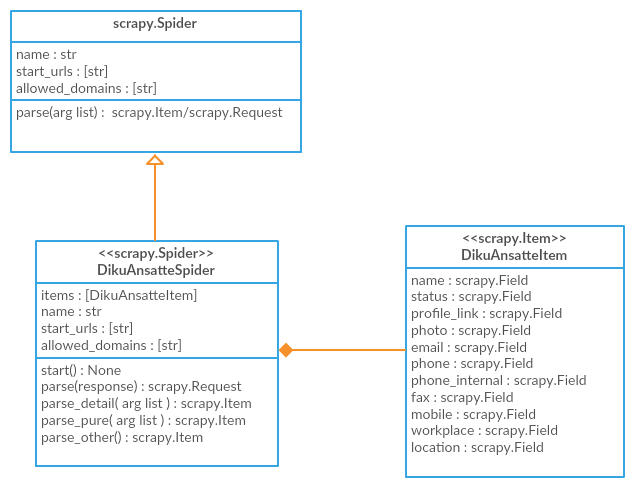
\includegraphics[scale=0.5]{scraper_class_diagram.png}
    \caption{Scraper klassediagram}
    \label{fig:scraper_class_diagram}
\end{figure}~\\
\hyperref[fig:scraper_class_diagram]{Figur \ref*{fig:scraper_class_diagram}} viser et UML-klassediagram over de klasser vi selv har implementeret (DikuAnsatteSpider og DikuAnsatteItem) og de Scrapy-klasser som de nedarver fra.\\
En såkaldt spider har en variabel, \texttt{name} repræsenteret som en streng. Denne bliver ikke specifikt brugt til noget, men er påkrævet af Scrapy.\\
\texttt{start\_urls} er liste af strenge, der beskriver hvilke URLs spideren skal starte med at høste data fra. Mindst én start-URL er påkrævet.\\
\texttt{allowed\_domains} er en liste af strenge der definerer hvilke domæner spideren er tilladt at høste fra.\\
\texttt{items} er en liste af \texttt{scrapy.Item}'s, som indeholder alle høstede "items", altså ansatte. Denne variabel kan så tilgås og manipuleres med, for at få fat i medarbejdernes kontaktinformation, lokation, navn, titel, osv.\\
\\
Der skulle også have været en scraper til at høste projektdata, men da der ikke er et samlet sted med alle projekter, kunne det ikke lade sig gøre.
% mere forklaring
\subsection{Frontend}
Under designet af vores frontend har der ikke været fokus på det æstetiske eller brugervenlighed, men i stedet på hvor meget information vi kan distribuere til de studerende. Vi påstår ikke at et flot og brugervenligt design ikke er vigtigt, men vi ville helst opfylde så mange krav så muligt, og æstetik var ikke en prioritet.\\
\\
Herunder har vi de mest essentielle sider i vores webapplikation.

\subsubsection{Projekter og vejledere}
\begin{figure}[H]
    \centering
    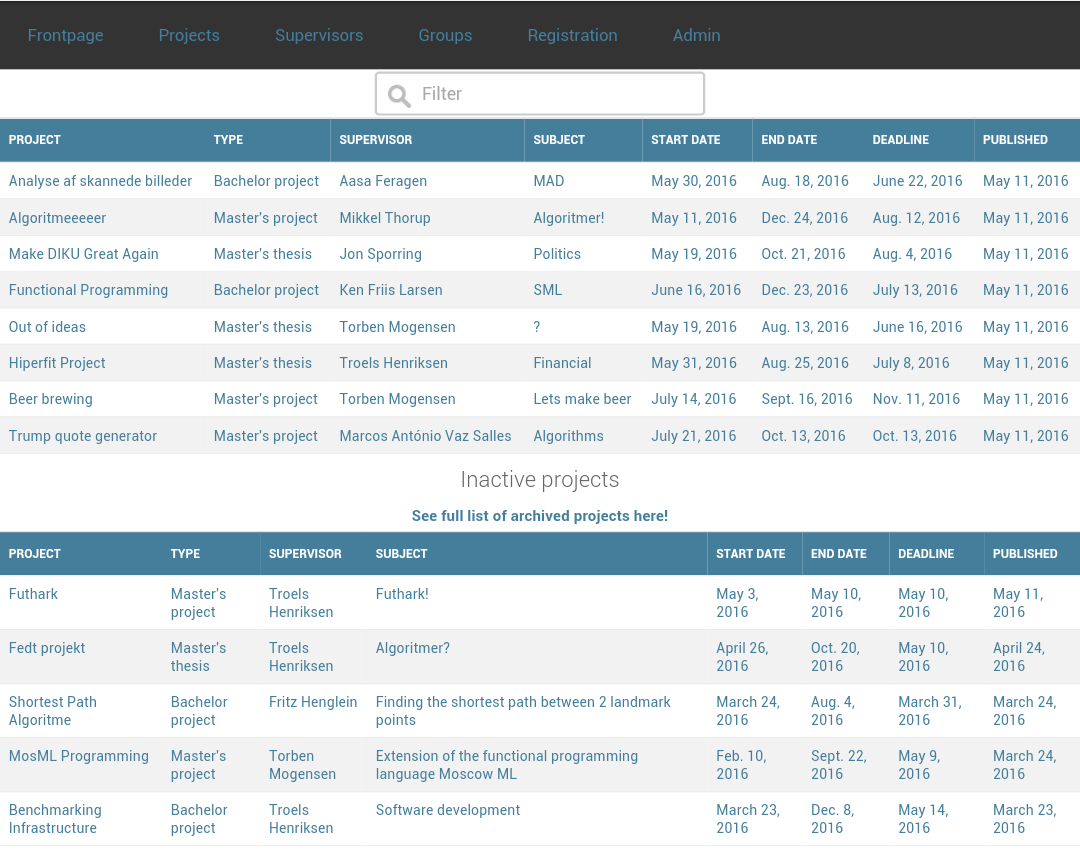
\includegraphics[scale=0.33]{frontend_projects.png}
    \caption{Oversigten over projekter på siden}
    \label{fig:frontend_projects}
\end{figure}
\begin{figure}[H]
    \centering
    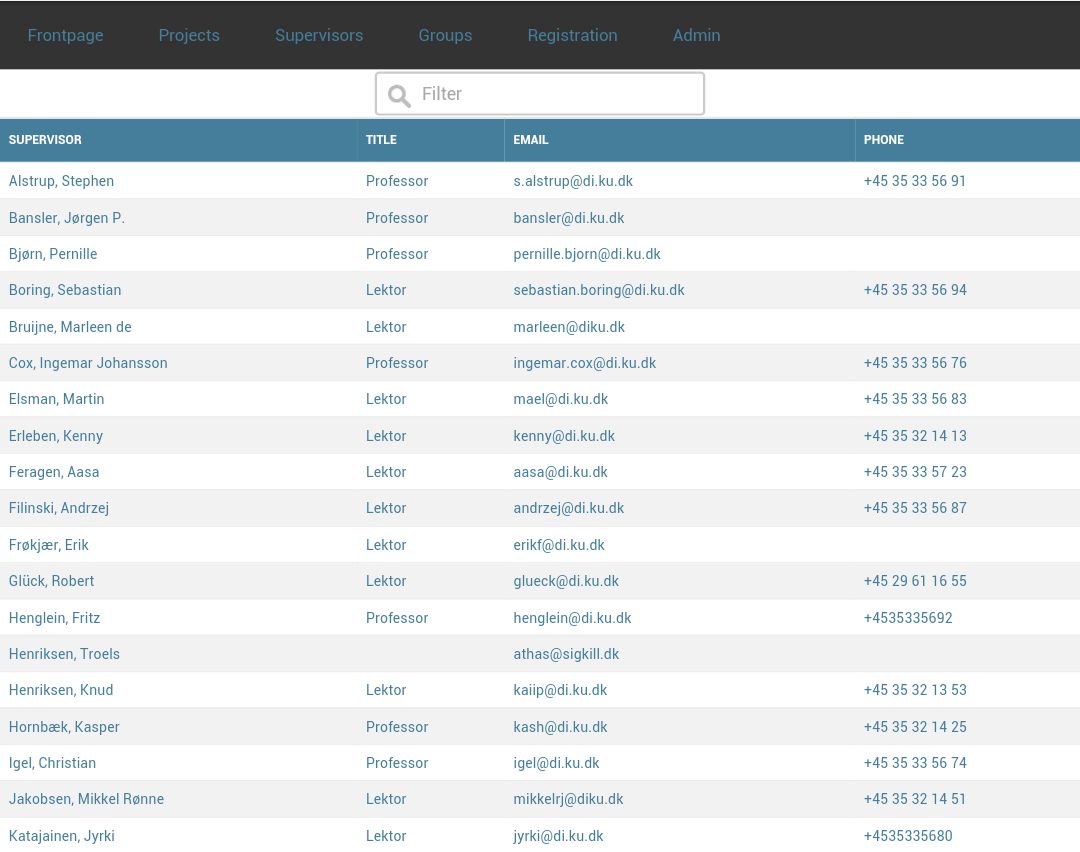
\includegraphics[scale=0.33]{frontend_supervisors.png}
    \caption{Oversigten over vejledere på siden (ikke alle vejledere kan ses på billedet)}
    \label{fig:frontend_supervisors}
\end{figure}
~\\
\hyperref[fig:frontend_projects]{Figur \ref*{fig:frontend_projects}} og \hyperref[fig:frontend_supervisors]{figur \ref*{fig:frontend_supervisors}} viser de to vigtigste sider i vores webapplikation. Disse to sider viser information omkring projekter og vejledere, og opfylder dermed henholdsvis krav 1 og 2 fra \hyperref[sec:corefuncs]{\ref*{sec:corefuncs}: \nameref*{sec:corefuncs}}. Klikker man på en vejleder eller et projekt, vil man blive vist detaljer omkring den specifikke vejleder eller projekt.

\subsubsection{Groups}
På denne side kan studerende se en oversigt over grupper med vejledere inden for et specifikt felt, og dermed finde adskillige vejledere inden for feltet, som den studerende interesserer sig for.
Denne side er funktionel og opfylder krav 1 under \hyperref[sec:nicefuncs]{\ref*{sec:nicefuncs}: \nameref*{sec:nicefuncs}}. Dog er scraperen endnu ikke i stand til også at høste ansattes grupper. \hyperref[fig:frontend_groups]{Figur \ref*{fig:frontend_groups}} på side \pageref{fig:frontend_groups} viser et screenshot af denne side.

\subsubsection{Registrering}
Her kan en vejleder registrere sig på siden, men kun hvis vejlederen allerede står som vejleder på siden, enten indhentet vha. scraperen eller indtastet manuelt af en "superuser". En superuser er en bruger på siden der kan tilføje, slette og redigere i alt.\\
Siden er ikke helt funktionel, da den ikke rigtigt gør noget, men dette ville ikke kræve meget ekstra arbejde at få lavet færdigt.
Denne side ville opfylde krav 3 fra \hyperref[sec:corefuncs]{\ref*{sec:corefuncs}: \nameref*{sec:corefuncs}}, hvis den havde været færdigimplementeret. \hyperref[fig:frontend_registration]{Figur \ref*{fig:frontend_registration}} på side \pageref{fig:frontend_registration} viser et udkast af denne funktion.

\subsubsection{Adminpanel}
Vi bruger Djangos indbyggede adminpanel, dog med nogle få ændringer, til at håndtere indtastning af data manuelt. Bl.a. er adminpanelet blevet udvidet med en navigationsbar til at navigere rundt på siden. Denne fulgte ikke med Djangos adminpanel, og det kunne derfor være svært at komme tilbage til vores webapplikation når man først går ind i adminpanelet. Screenshots af adminpanelet, med og uden ændringer, kan ses på \hyperref[fig:frontend_admin_vanilla]{figur \ref*{fig:frontend_admin_vanilla}}, \ref{fig:frontend_admin_login} og \ref{fig:frontend_admin} i \nameref{sec:bilag_frontend}.

\section{Afprøvning}
\label{sec:afproevning}
\subsection{Acceptance tests}
Til afprøvning og test af projektet gjorde vi os nogle forskellige overvejelser. Vi var bl.a. i tvivl om hvorvidt vi skulle anvende Fitnesse eller Robot frameworket. Vi endte med at bruge Robot til at skrive automatiske acceptance-tests. I samspil med Robot, bruger vi et bibliotek kaldt \textit{Selenium2Library}, som gør det muligt at tilgå elementer på hjemmesider vha. HTML og XML.
Disse tests er yderligere beskrevet i \nameref{sec:bilag_tests}.

\subsection{Videreudvikling og vedligeholdelse}
Vi har valgt ikke at sikre applikationens opfyldelse af krav ved tests. Dette er grundet, at vi prioriterede færdigudvikling af projektet over hvad vi vil mene er overflødig test. Her menes der, at vi kan se at hjemmesiden opfylder de stillede krav fra sektion \hyperref[sec:krav]{\ref*{sec:krav}: \nameref*{sec:krav}}. Det ved vi, da vi har brugt hjemmesiden ved manuelt at bevæget os rundt og løbende opdaget fejl og mangler, og derefter rettet/implementeret dem. \\
Til fremtidig brug er vores acceptance-tests skrevet således, at selvom der skulle opstå ændringer på hjemmesiden, kan vi nemt bruge dem igen. Dette er fordi de tilgår elementer i den tabel, som hjemmesiden repræsenterer information i, i stedet for at tilgå de specifikke elementer cellerne indeholder. For testen er det altså ligegyldigt hvad der står i tabellen, bare siden har samme struktur. Skulle selve strukturen af sitet dog ændres, kan vi forholdsvis nemt omskrive testene til at tilgå elementer på en ny måde, da det blot er kodedelen der beskriver hvilket element der skal tilgås, som skal omskrives. \\
Da vores tests, som beskrevet ovenfor, er forholdsvis automatiske og agile, kan vi nemt anvende dem når vi tilføjer ting til sitet, eller ændrer på de ting som i forvejen er til stede. Det har givet mulighed for ubesværet at teste, mens vi har arbejdet på projektet. \\

\subsection{Unit-tests}
Selvom vi bruger Django, hvilket er et omfattende og stabilt framework, har vi valgt at unit-teste dele af projektet, for at sikre fejlbarheden så vidt som muligt. Django-funktionerne har vi i grove træk testet ved at opsætte to scenarier for de forskellige framework-funktioner, ét scenarie som får forkerte specifikationer og ét scenarie som får de korrekte. Således kan vi se om de fejler eller kører som ønsket og forventet. Disse tests er også yderligere beskrevet i \nameref{sec:bilag_tests}.

\subsection{Kørsel af test}
For at efterprøve vores tests, kan de køres på følgende vis
\begin{enumerate}
  \item Installer Robot vha. pip installer og følgende kommando\\
  \texttt{pip install robotframework}
  \item Find ind i test mappen via følgende sti \\ \texttt{ProjectStockSD/project\_stock/project\_stock/tests/RobotTests/real\_tests} 
  \item Kør den valgte test ved at skrive \texttt{robot valgte test} eksempelvis
  \texttt{robot ProjectsTest.robot}
  \item Hvis robot er installeret korrekt skulle terminalen gerne se således ud 
    \begin{figure}[H]
        \centering
        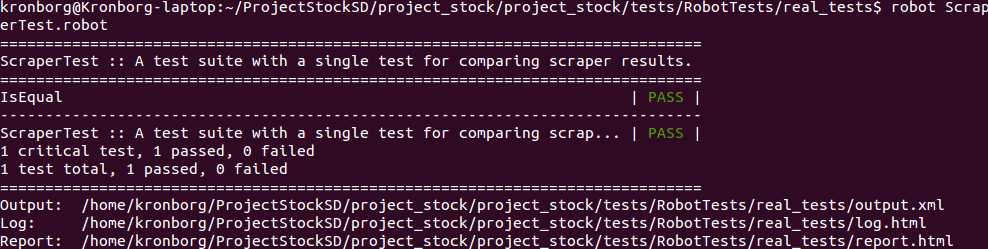
\includegraphics[scale=0.5]{test.png}
        \caption{Konsol output efter robot test}
        \label{fig:console output}
    \end{figure}~
  \item Yderligere kan man se udvidet information om testen i de generede filer \texttt{log.html} og \texttt{report.html}. Uddrag af disse kan også findes i \nameref{sec:bilag_tests}.
\end{enumerate}
\section{Udviklingsmiljø}
\label{sec:udvikling}
Vi vil i dette afsnit beskrive vores opsætning af versionsstyring og struktur for projektet. Endvidere hvilke værktøjer vi har brugt og hvordan vi har brugt dem.

\subsection{Opsætning og struktur}
Vi har brugt versionsstyringsværktøjet \textit{Git} til dette projekt. Git holder styr på de filer man lægger ind i sit \textit{repository}. Et repository er i en software udviklingssammenhæng en mappe hvori man gemmer alle de filer, som tilsammen udgør et projekt. Hver udvikler har et lokalt repository, som skubbes til et offentligt repository når man er færdig med at kode. Git holder styr på filernes versioner og sørger for, at forskellige versioner kan flettes sammen, i tilfælde af at to udviklere har skrevet i samme fil.\cite{git}\\
\\
Vores repository er struktureret således, at vi gemmer vores rapporter og andet i en separet mappe fra selve vores produkt, men dog stadig i samme repository. På denne måde kan vi også bruge versionsstyring til at skrive dokumentation og rapporter sammen.

\begin{figure}[H]
	\centering
	\includegraphics[scale=0.55]{repostruct.png}
	 \caption{Abstrakt struktur af vores repository}
	 \label{fig:repostruct}
\end{figure}
~\\
\hyperref[fig:repostruct]{Figur \ref*{fig:repostruct}} viser strukturen af vores repository. Vi har valgt at lave figuren abstrakt og undladt visse mapper, primært fordi vi skriver i frameworket Django, som har en del filer og mapper som skal være der, men som vi ikke rigtig selv har brugt særligt meget. Filen \texttt{manage.py} er som tidligere nævnt vigtig, og er derfor inkluderet. Hjemmesiden indeholder en masse Django specifikke filer som f.eks. et database schema, skabeloner til selve hjemmesiden og meget andet.

\subsection{Udviklingsmiljø}
Vi har til projektet besluttet ikke at bruge et specifikt IDE (Integrated Development Environment) til at udvikle i. Grunden til dette er, at vi alle har forskellige præferencer og arbejder bedst på forskellige måder. Nogen af os vil gerne have en simpel IDE, såsom Emacs, som ikke kan så meget fra starten af, men hvor man kan tilføje funktioner og værktøjer for at tilpasse IDEen, bl.a. for at optimere ens effektivitet, men også for samtidig at undvære unødvendige funktioner. Andre fra gruppen ville hellere have en større IDE, såsom Atom, som fra start kan en hel del mere. \\
\\
Vi besluttede os for at vi hver især arbejder mere effektivt og bedre, hvis vi udvikler det der passer os bedst indviduelt. Det vil sige, at nogle medlemmerne af vores gruppe selv har stået for at kunne afprøve programmet, lave refaktorering og afvikling af hjemmesiden. At kunne gøre brug af værktøjer til refaktorering, har ikke været et stort problem til vores projekt, da måderne at gøre ting på i Django, er meget specifikke. Derfor skal klasser, funktioner og andet se ud på en meget bestemt måde, hvilket vi fik sørget for i første omgang.

\subsection{GitHub}
Vi har brugt GitHubs \textit{issue tracking system}\cite{issuetracking} og tildelt issues milepæle, for at holde styr på hvilke arbejdsopgaver eller use cases, vi gerne vil have klaret inden en given iteration er færdig. Milepælene svarer til delafleveringerne og den endelige rapport. Derudover har vi en ekstra milepæl, som bliver brugt til at holde styr på opgaver, vi godt kunne tænke os at implementere, men som ikke er strengt nødvendige. Denne milepæl har vi kaldt "nice to haves."{} Et medlem kan derfor sætte sig selv (eller andre) på en opgave, så alle andre kan se hvem der arbejder på hvad. Der kan læses mere om, hvordan vi har brugt Git og hvilke udfordringer vi har haft i afsnit \ref{sec:git}.

\section{Diskussion og reflektion} % Alle
\label{sec:diskussion}

\subsection{Udviklingsprocessen}
Vi har som gruppe bestræbt os på at mødes mindst én gang om ugen. Dette selvorganiserede møde er udover de ugentlige møder med instruktorerne. På disse selvorganiserede ugentlige møder har vi uddelegeret arbejdsopgaver og diskuteret og arbejdet med forskellige værktøjer og frameworks.\\
Disse møder har fungeret godt, og det har været mere effektivt at kunne kommunikere ansigt til ansigt i stedet for skriftligt.

\subsection{Git}
\label{sec:git}
Vi har igennem projektet arbejdet meget med Git, herunder den online service GitHub, og dermed lært en del om Git. I starten af forløbet fik vi mange \textit{merge commits}. Git gemmer ændringer i commits, og en merge commit er en sammenfletning af to commits. Merge commits opstår når flere har foretaget ændringer i samme fil og ikke arbejder ud fra seneste commit. Git skal derfor flette de ændrede filer fra begge udviklere sammen.\\
\\
Vi undersøgte problemet, og fandt frem til nogle Git-opsætninger som hjalp med at undgå disse merge conflicts.\cite{mergecommits}\\
\\
Vi har ligeldes benyttet flere af GitHubs forskellige funktionaliteter til intern kommunikation. I roden på vores GitHub repository findes filen \texttt{README.md}. Denne fil har været brugt til vidensdeling.
Her har vi bl.a. skrevet tips til at bruge Git mere effektivt og til at dele tanker og generelle informationer, der er relevante for projektet. Dette kan være alt fra, hvilke hjemmesider vi kan scrape, og hvordan man kan scrape det, til at dele YouTube videoer, der beskriver Django. \\ \\
% teksten herunder er næsten identisk med GitHub afsnittet under Udviklingsmiljø
Vi benyttet GitHub til at holde styr på arbejdsopgaver, som minder om use cases. Dette er gjort ved at oprette milepæle og \textit{issues}, milepælene er blevet sat til de forskellige delafleveringer/iterationer, inkl. den endelig rapport og en ekstra milepæl til 'nice to have' features. Derefter er der blevet oprettet issues til hver milepæl som afspejler hvad vi gerne vil have lavet færdig inden den næste iteration. Derved kan vi også holde styr på hvem laver hvad, da man kan tilføje medlemmer af gruppen til et issue, men man kan også diskutere løsninger og andet, selvom vi ikke sidder sammen og arbejder.
Vores issues minder om use cases, men de kan også være bugs eller anden implementation som ikke nødvendigvis er en use case. \\
\\
Igennem forløbet har vi været gode til at få lavet de opgaver vi havde sat os for at skulle løse, selvom der er nogle enkelte issues, som ikke er blevet lukket inden forløbets afslutning. Disse implementationer har vi valgt at beskrive senere i rapporten. \\ \\
Vi begyndte først rigtig at bruge de her GitHub-funktioner, såsom issues og milepæle, efter 1-2 måneder inde i forløbet. Set tilbage ville vi gerne have startet med det tidligere, da det maksimerer effektivitet, men vi kendte simpelthen ikke til det på det tidspunkt, og fik det faktisk anbefalet af en anden gruppe til en review-session. % reference til bilag?

\subsection{Testing}
\subsubsection{Test-first og test-driven development}
I vores arbejde med projektet, har vi hverken benyttet princippet \textit{test-first} eller \textit{test-driven development (TDD)}, der b.la. kendes fra metodologien \textit{Extreme Programming (XP)}. Test-first og TDD består af at lave tests, og dermed får fastlagt programmets og klassers struktur inden man begynder at kode.\\
\\
Vi har senere erfaret, at det kunne have været nyttigt i visse tilfælde, hvis vi havde benyttet en test-first tilgang. Dels fordi det ville være nemmere at unit teste vores kode, og dels fordi det formentlig havde ført til at vi havde skrevet kode, der var mere afkoblet. \\
Vores begrundelse for ikke at benytte test-first, var at det var svært at forene med Django frameworkets faste krav for, hvordan koden skal struktureres. \\
Derimod kunne vi godt have have benyttet en test-first tilgang til vores web scraper.

\subsection{Web scraper}
Den web scraper vi har udviklet, er designet til at høste data fra siden \url{http://diku.dk/Ansatte}, samt profilsiderne for Datalogisk Instituts ansatte. Der linkes til disse profilsider fra \url{http://diku.dk/Ansatte}.\\
Vi har vurderet, at det ville være svært og formentlig unødigvendigt at designe en abstrakt scraper, som ville være i stand til at høste data fra mange forskellige websteder. At ekstrahere data fra et specifikt websted, afhænger i høj grad af, hvordan dette websted er opbygget. Er den information man er interesseret i, f.eks. placeret i  HTML-tabeller, skal man vide hvilke HTML-tags og -attributer man skal lede efter. Ligeledes skal man vide, hvordan denne information er formateret. \\
Da vi ikke har fundet andre websteder, hvor man kan høste information om de ansatte, eller projekter, for den sags skyld, vurderede vi at ikke ville være i overenstemmelse med den agile tankegang at prøve at designe en abstrakt scraper.

\subsection{Distrubution af arbejdet}
<<<<<<< HEAD
Arbejdet med projektets forskellige elementer er blevet fordelt således, at hvert element er blevet udført af en eller to af gruppens medlemmer. En fordel ved denne metode er, at det er nemmere at uddelegere arbejdet, og at gruppens medlemmer skal fokusere på færre ting. Men samtidig kan det betyde at koden kan indeholde flere fejl. Ligeledes kan det betyde at det kan være sværere for udefrakommende personer eller de andre gruppemedlemmer at forstå de enkelte dele af projektet. Da man kan tendens til at skrive enten kode eller rapport på en måde, der kun er foreståelig for en selv.
=======
Arbejdet med projektets forskellige elementer er blevet fordelt således, at hvert element er blevet udført af en eller to af gruppens medlemmer. En fordel ved denne metode er, at det er nemmere at uddelegere arbejdet, og at gruppens medlemmer skal fokusere på færre ting. Men samtidig kan det betyde at koden kan indeholde flere fejl. Ligeledes kan det betyde at det kan være sværere for udefrakommende personer eller de andre gruppemedlemmer at forstå de enkelte dele af projektet, da man kan have en tendens til at skrive enten kode eller rapport på en måde, der kun er foreståelig for én selv.
>>>>>>> d5d0e77e45b7f14eb10f913cdd6c9caddccb6356

\section{Videreudvikling}
\label{sec:videreudvikling}
Vi vil diskutere de krav vi ikke nåede at implementere, men som vi gerne ville have lavet, givet mere tid. Dette kan ses som en liste over use cases, som et hold af udviklere skulle modtage, hvis de overtog projektet efter os.\\
Bemærk at nedenstående ikke er use cases, men en beskrivelse af de ting der skal være en del af de use cases, som udviklerne skulle tilsendes.\\
\begin{itemize}
\item Verifikation og oprettelse af vejledere i systemet. Vi nåede ikke at lave et færdigt system til at lade vejledere registere sig i vores system, så de selv kan ligge projekter op på hjemmesiden.
\item Man skal kunne se en liste over publikationer hos en vejleder, og en vejleder skal kunne ligge publikationer ind på sin side.
%tilføj mindst en mere
\end{itemize}

\newpage
\section{Konklusion}
\label{sec:konklusion}
% Christian

\newpage
\begin{thebibliography}{9}

\bibitem{agile}
	Martin, R.C., Martin, M.,
	\emph{Agile Principles, Patterns, and practices in C\#},
	Upper saddle river, NJ, Prentice Hall,
	2007

\bibitem{cc}
	Steve McConnell,
	\emph{Code Complete},
	2nd edition,
	2004.

\bibitem{djangoFAQ}
	\url{https://docs.djangoproject.com/en/1.9/faq/general/}

\bibitem{djangoView}
	\url{https://docs.djangoproject.com/ja/1.9/topics/http/views/}

\bibitem{djangoTemplate}
	\url{https://docs.djangoproject.com/en/1.9/topics/templates/}

\bibitem{scraping}
    \url{https://en.wikipedia.org/wiki/Web_scraping}

\bibitem{models}
    \url{https://docs.djangoproject.com/en/1.9/topics/db/models/}

\bibitem{git}
    \url{https://en.wikipedia.org/wiki/Git_(software)}

\bibitem{figure_djangoadmin}
    \url{http://www.djangobook.com/en/2.0/chapter06.html}
\bibitem{issuetracking}
    \url{https://en.wikipedia.org/wiki/Issue_tracking_system}

\bibitem{mergecommits}
    \url{https://github.com/cenh/ProjectStockSD/blob/0.1.1/README.md#undgå-merge-commits}
% der skal også datoer på links

\end{thebibliography}

\newpage
\section{Bilag}
\label{sec:bilag}

\subsection{Bilag A}
\label{sec:bilagA}
\begin{center}
	\begin{tabular}{|p{0.05\textwidth}|p{0.5\textwidth}|p{0.45\textwidth}|}
		\hline
	\textbf{D\#} & \textbf{Færdigimplementerede use cases} & \textbf{Ændringer i designet} \\ \hline

	D1 & Vi fik ikke færdiggjort nogen use cases i dette \textit{sprint}. & Ingen ændringer, da projektet påbegyndes her. \\ \hline

	D2 & 		\begin{minipage}[t]{0.4\textwidth}
	\begin{itemize}
		\item Det skal være muligt at se et katalog over projekter.
		\end{itemize}
		\end{minipage} & Vi begyndte at bruge Django (web framework). Vi tog dette valgt, efter at have snakket med andre grupper, og foretaget \textit{research} på nettet. Vi mente, at det kunne hjælpe os med at opfylde vores use cases. \\ \hline

	D3 &
	\begin{minipage}[t]{0.4\textwidth}
	\begin{itemize}
		\item Systemet skal kunne præsentere \textit{up-to-date} oplysninger om potentielle vejledere, herunder:
		\begin{itemize}
			\item Tidligere projekter.
			\item Forskningspublikationer.
			\item Kontaktoplysninger.
		\end{itemize}
	\end{itemize}
	\end{minipage} & k \\
		\hline
	D4 & k & k \\ \hline
	\end{tabular}
\end{center}~\\

\subsection{Bilag B}
\label{sec:bilagB}
% Lasse
Arkivet \texttt{Exam.zip} er vedlagt og indeholder alt der skal bruges for at køre webapplikationen.
Alternativt kan arkivet hentes her:\\
\url{https://github.com/cenh/ProjectStockSD/archive/0.1.1.zip}


\subsection{Bilag C}
\label{sec:bilagC}
\subsubsection{R1: Krav}

\subsubsection*{\textit{Meta:}}
Vi foretog i dette \textit{sprint} et \textit{review} af 'gruppe 4's delaflevering 1. Her gav vi dem følgende kommentarer, her præsenteret som stikord til os selv, der blev uddybet, mundtligt.

\subsubsection*{\textit{Review:}} 
\textbf{Afklaring af krav} \\
Beskriver den nuværende problemstilling fint ("shopping" problemet).
<<<<<<< HEAD
User stories: \\
- Hvad med business-clubs?\\
\textbf{Opsætning af udviklingsmiljø} \\
Udførlig beskrivelse.\\
\textbf{Den næste iteration} \\
- Uklart hvornår en underopgave, knyttet til en user story, er godkendt. Menes der her tests der passeres? \\
- Lidt uklare termer for uindvidede ("Forbind dette nye view med et url.") \\
- Underopgaverne til use case 1 og 2 er nærmest identiske. \\
- Use case 3(a), hvad menes med: "Tjek at databasens "Counselor" model har \\ kontaktoplysninger, tilføj og tilpas efter behov." \\
- Use case 3(c), hvilke informationer skal mere præcist være knyttet til en vejleder.\\
\textbf{Generelt} \\
- Generelt virker de \textit{use cases} I har valgt at implementere i næste iteration overkommelige, udfra hvad I hidtil har nået. \\
=======
User stories:
- Hvad med business-clubs?
\textbf{Opsætning af udviklingsmiljø}
Udførlig beskrivelse.
\textbf{Den næste iteration}
- Uklart hvornår en underopgave, knyttet til en user story, er godkendt. Menes der her tests der passeres?
- Lidt uklare termer for uindvidede ("Forbind dette nye view med et url.")
- Underopgaverne til use case 1 og 2 er nærmest identiske.
- Use case 3(a), hvad menes med: "Tjek at databasens "Counselor" model har kontaktoplysninger, tilføj og tilpas efter behov."
- Use case 3(c), hvilke informationer skal mere præcist være knyttet til en vejleder.
\textbf{Generelt}
- Generelt virker de use cases I har valgt at implementere i næste iteration overkommelige, udfra hvad I hidtil har nået. \\
>>>>>>> d5d0e77e45b7f14eb10f913cdd6c9caddccb6356
- I har ikke lagt fokus på høstning af data. I nævner ikke eksplicit, hvor jeres data kommer fra. \\
- Verificering af vejledere. Loginsystem?

\subsubsection{R2: Design}
\subsubsection*{\textit{Meta:}}
Vi foretog i dette \textit{sprint} et \textit{review} af 'gruppe 4's delaflevering 2.

\subsubsection*{\textit{Review:}}
Afsnittet "Afprøvning" er godt. \\
Jeres test-metoder er veldokumenterede. \\
Figur 2 i afsnittet "Abstraktion og designmønstre" er lidt forvirrende og misvisende. \\
Tabllen, der indeholder hvilke brugere, der har hvilke rettigheder i underafsnittet "CRUD-modellen" hjælper meget på forståelsen.

\subsubsection{R3: Kode}
\subsubsection{R4: Release}

\newpage
\subsection{Bilag D}
\label{sec:bilag_tests}
\subsubsection*{Acceptance-tests}
\begin{center}
	\begin{tabular}{|p{0.08\textwidth}|p{0.44\textwidth}|p{0.44\textwidth}|}
		\hline
	\textbf{Test\#} & \textbf{Testbeskrivelse} & \textbf{Testresultat} \\ \hline

	Test 1 & Denne test består af et \textit{Robot}-script som finder alle "clickable links" på siden der viser projekter, og sikrer at disse henviser til de rigtige steder. Den tjekker om det passer ved at sammenligne den side den ender på, med den side vi mener det skulle være & Scriptet klikker på alle 104 links, og ser at de alle henviser som de skal og returnerer "\textit{All tests passed}"{} i \textit{Robot}-rapporten.\\ \hline

	Test 2 & Denne tests funktion er at teste om man kan tilgå vejledere fra vejleder siden, og om disse informationer er vist korrekt. Som eksempel bruger vi navnet "Torben", scriptet går så listen af vejledere igennem, finder et resultat i tabellen hvor "Torben" indgår, og tager et screenshot af Torbens informationer. & Denne test er lidt mere manuel da den kræver at vi gennemser oplysningerne fra screenshottet. Men \textit{Robot} returnerer at testen er passed, da det lykkes den at finde en vejleder ved navn "Torben" og tage et screenshot af hans side.\\ \hline

	Test 3 & Denne test hjælper på sin vis den forhenværende test. Dens funktion er at sikre at de scrapede informationer er korrekte. Det gør den ved først at gå ind på Diku's hjemmeside og finde oplysninger på en vejleder. Herefter går den så på vores side, finder samme vejleder og ser om de 2 stykker information er de samme ved en \textit{Robot}-funktion kaldt \textit{IsEqual} & Denne test som den eneste returner en bool, og da denne er true, viser det at de to stykker information er sande, og scraperen derfor virker korrekt. \newline
	Ligeledes hjælper det os med, ikke at skulle tjekke test 2 manuelt, når vi ved at de oplysninger der fremgår på siderne er sande. \\ \hline
	\end{tabular}
\end{center}
\newpage
\subsubsection*{Unit-tests}
\begin{center}
	\begin{tabular}{|p{0.08\textwidth}|p{0.44\textwidth}|p{0.44\textwidth}|}
		\hline
	\textbf{Test\#} & \textbf{Testbeskrivelse} & \textbf{Testresultat} \\ \hline

	Test 1 & Den første test tester om Django generer projekter korrekt. Det gør vi ved at give den kombinationer af inputs, så der er fejlbare projekter og korrekte projekter. Vi beder så Django generere projekter baseret på både de fejlbare og korrekte informationer, og vi ser så at funktionerne fejler og kører som ønsket. & Resultaterne for denne test er simple. Funktionerne returnerer den ønskede kombination af true og false, og vi kan se at de virker som ønsket.  \\ \hline

	Test 2 & Denne test sikrer at delene på \textit{Supervisor}-siden bliver generet af Django korrekt. På samme måde som test 1, giver vi Django 2 sæt oplysninger. Ét som gør det muligt for funktionerne at køre, og ét der ikke gør. På denne måde kan vi se hvilke dele der gør det muligt, og hvilke dele der forhindrer Django i at køre som ønsket. &  Resultaterne for denne test, er ligesom test 1. De returnerer true og false som forventet, og dette viser at Django's funktioner er korrekte. \\ \hline

	Test 3 & Den sidste unit-test tester om Django kan tilgå sig selv, ved at sende requests til de forskellige dele af projektet og returnerer true hvis den får det rigtige output. Den består af fem underfunktioner, som tilgår de forskellige primære views. Hver af disse funktioner returner en "status\_code" som fortæller hvordan funktionen forløb. Hvis denne status\_code er i mellem 200 og 400 betyder det at henvisningen er som ønsket. & Ved gennemløb af alle requests ser vi de forskellige funktioners "status\_code" værdier, og da de alle returnerer værdier imellem de ønskede 200 - 400, passerer testen. \\ \hline
	\end{tabular}
\subsubsection*{Robot resultater}
    \begin{figure}[H]
        \centering
        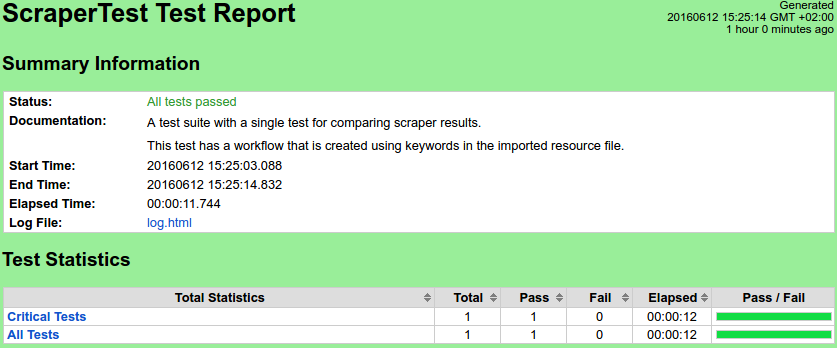
\includegraphics[scale=0.5]{report.png}
        \caption{Robot testens rapport}
        \label{fig:robot report}
    \end{figure}
    \begin{figure}[H]
        \centering
        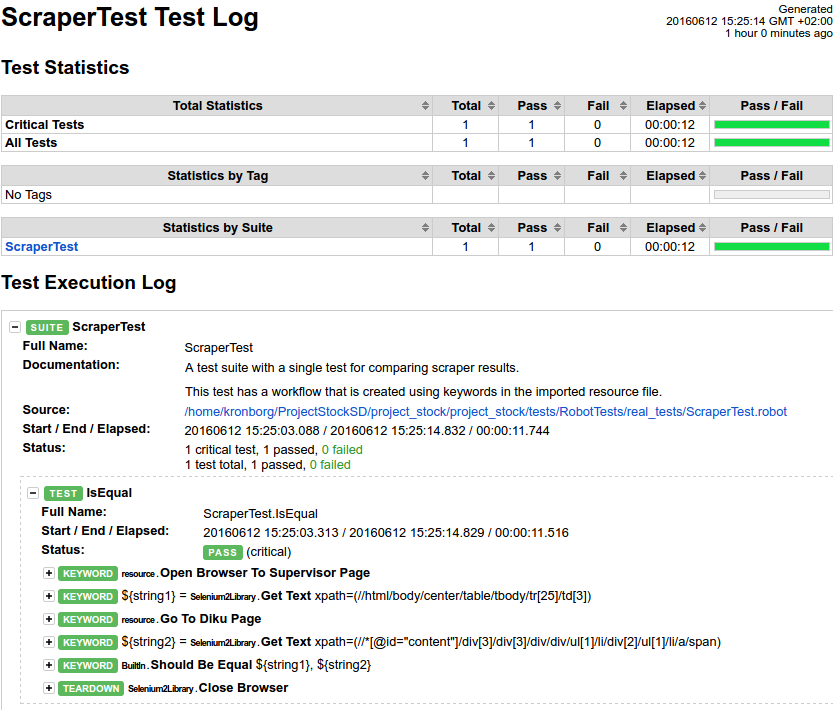
\includegraphics[scale=0.5]{log.png}
        \caption{Robot testens log}
        \label{fig:robot log}
    \end{figure}
\end{center}

\subsection{Bilag E}
\label{sec:bilag_struktur}
Strukturen i vores Django-projekt er vist herunder.\\
\texttt{\_\_init\_\_.py} filer er udeladt, samt andre filer der ligner hinanden.\\
Se evt. vedlagte arkiv \texttt{Exam.zip}.
\begin{nodeC}
    \item{project\_stock}
    \begin{nodeC}
        \item{manage.py}
        \item{project\_stock}
        \begin{nodeC}
            \item{admin.py}
            \item{apps.py}
            \item{fillmockdata.py}
            \item{forms.py}
            \item{models.py}
            \item{scrapers}
            \begin{nodeC}
                \item{dikuspider.py}
            \end{nodeC}
            \item{settings.py}
            \item{templates}
            \begin{nodeC}
                \item{...}
            \end{nodeC}
            \item{templatetags}
            \begin{nodeC}
                \item{project\_stock.py}
            \end{nodeC}
            \item{tests}
            \begin{nodeC}
                \item{RobotTests}
                \begin{nodeC}
                    \item{...}
                \end{nodeC}
                \item{test\_models.py}
                \item{test\_views.py}
            \end{nodeC}
            \item{urls.py}
            \item{views.py}
            \item{wsgi}
        \end{nodeC}
        \item{static}
        \begin{nodeC}
            \item{...}
        \end{nodeC}
        \item{templates}
        \begin{nodeC}
            \item{...}
        \end{nodeC}
    \end{nodeC}
\end{nodeC}

\subsection{Bilag F}
\label{sec:bilag_frontend}
\begin{figure}[H]
    \centering
    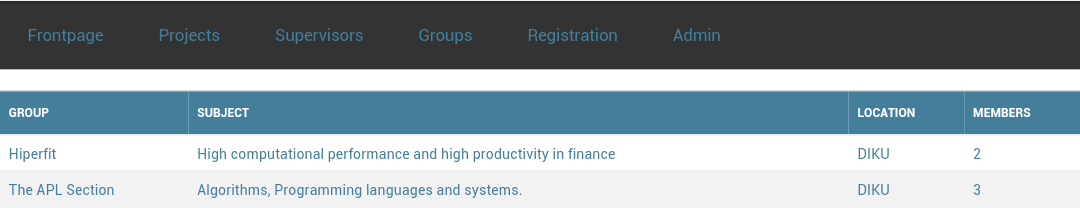
\includegraphics[scale=0.33]{frontend_groups.png}
    \caption{Oversigten over grupper på siden}
    \label{fig:frontend_groups}
\end{figure}
\begin{figure}[H]
    \centering
    
\includegraphics[scale=0.33]{frontend_registration.png}
    \caption{Registrering af vejledere}
    \label{fig:frontend_registration}
\end{figure}
\begin{figure}[H]
    \centering
    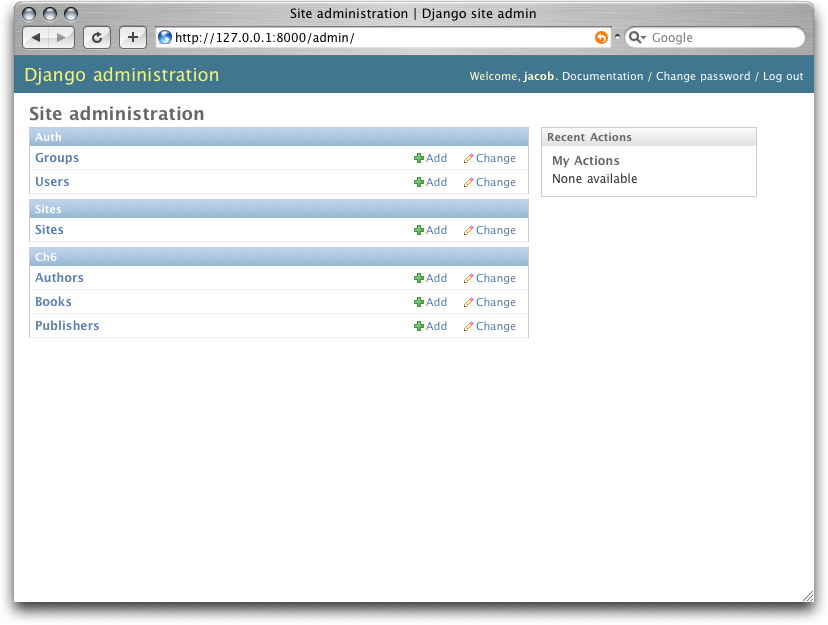
\includegraphics[scale=0.5]{frontend_admin_vanilla.png}
    \caption{Adminpanel uden ændringer\cite{figure_djangoadmin}}
    \label{fig:frontend_admin_vanilla}
\end{figure}
\begin{figure}[H]
    \centering
    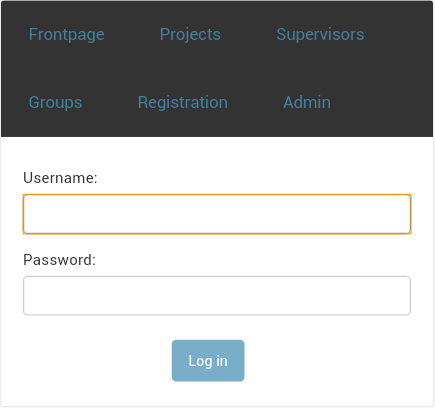
\includegraphics[scale=0.5]{frontend_admin_login.png}
    \caption{Adminpanelets login-side med navigationsbar tilføjet}
    \label{fig:frontend_admin_login}
\end{figure}
\begin{figure}[H]
    \centering
    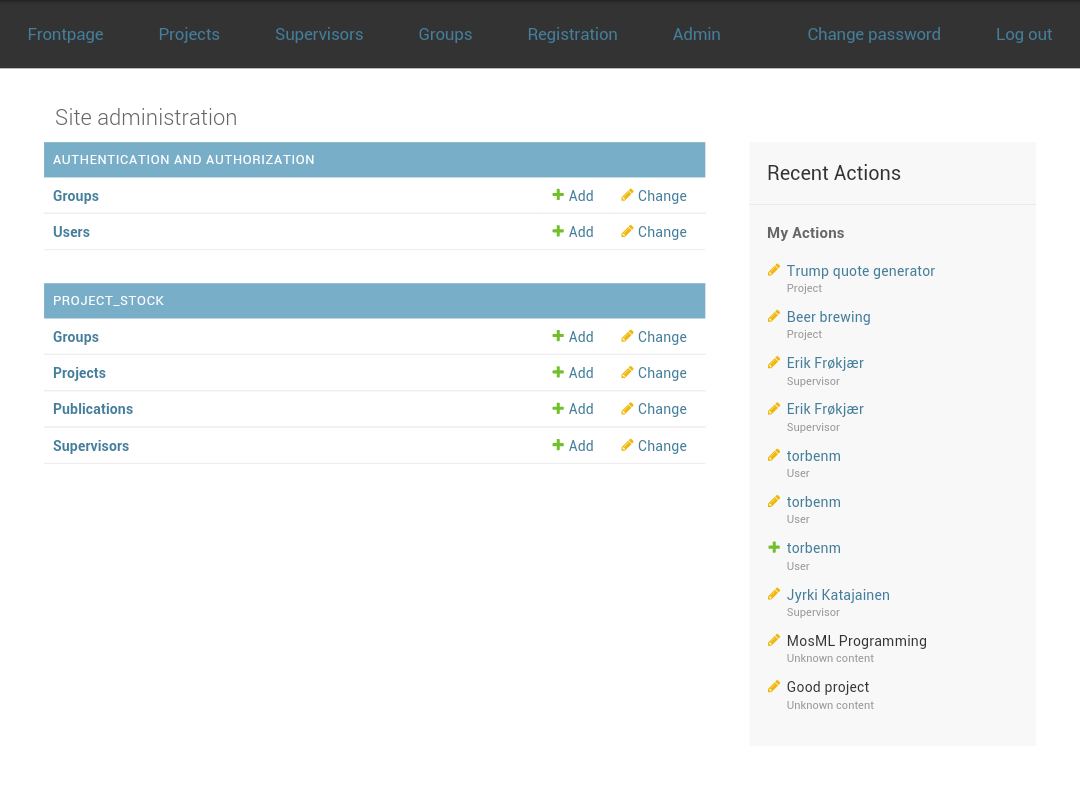
\includegraphics[scale=0.35]{frontend_admin.png}
    \caption{Adminpanelet efter login}
    \label{fig:frontend_admin}
\end{figure}
\end{document}
